\subsection{Multiplication matrice vecteur creuse}
La multiplication du matrice creuse par un vecteur est une opération dont le ratio nombre d'opérations par le nombre d'octet lus est petit.
%
Dans le cas d'une matrice scalaire, ce ratio vaut environ $1/10$ en double précision.
%
Pour chaque valeur non-nulles de la matrice, il faut lire cette valeur, l'indice de la colonne et la valeur contenue dans le vecteur à l'indice de la colonne.
%
Il faut ensuite multiplier les deux valeurs ensemble et l'ajouter à un accumulateur, ce qui fait en double précision 2 opérations pour 20 octets lus.
%
Si nous utilisons trois variables primaires, chaque entrée de la matrice est un bloc 3 par 3.
%
Nous devons donc lire ce bloc (9*8 Octets), lire l'indice de colonne (4 Octets) et finalement lire 3 valeurs dans le vecteur (3*8 Octets).
%
Pour chaque valeur du bloc nous avons 2 opérations à faire (2*9), nous avons donc un ratio de $18/100$ soit environ $1/5,5$.
%
Avec huit variables primaires, le ratio monte à environ de $1/4,5$.


Le {\em roofline model} est un modèle de performance permettant de connaître la puissance de calcul maximale pouvant être atteinte par un algorithme sur une machine.
%
Ce modèle se construit de la façon suivante, dans un premier temps nous allons mesurer la bande passante maximale de la machine.
%
Pour cela nous avons utilisé le benchmark STREAM, sur Rostand, nous obtenons une bande passante de 21~Go/s.
%
Puis, dans un second temps, nous allons calculer la capacité de calcul maximale de la machine.
%
Pour calculer cette capacité, il faut multiplier le nombre de coeur de calcul par le nombre maximal d'opérations faites dans une instruction et multiplier le tout pas la fréquence d'horloge.
%
Chaque noeud de Rostand étant composé de 12 coeurs cadencés à 2,80~GHz et du jeu d'instructions SSE~4.2 permettant d'effectuer 4 opérations flottantes en simple précision à la fois, ce qui donne 134,4~GFlops.
%
Le nombre d'opérations simultanées en double précision est divisé par 2, donc on peux avoir au maximum 67,2~GFlops et si nous n'utilisons pas le jeu d'instructions vectorielles, nous pouvons obtenir au maximum 33,6~GFlops (Fig.~\ref{fig:roofline_rostand}).


Une fois le roofline model construit, nous pouvons donc placer le produit matrice vecteur creux.
%
Les performances du SpMV dépendent du nombre de variables primaires, nous avons donc placé sur le roofline model trois SpMV en fonction du nombre de variable primaire utilisées.
%
Ces trois points nous indiquent que les performances du SpMV seront limitées par la bande passante mémoire.
%
L'utilisation du jeu d'instructions vectorielles aura donc très peu d'impact sur nos performances.
%
Nous devons nous concentrer sur les accès mémoires et surtout dans notre cas, sur les effets NUMA.


Le SpMV présente du parallélisme de boucle sur les lignes de la matrice.
%
Nous pouvons multiplier indépendamment chaque ligne de la matrice par un vecteur et stocker directement le résultat dans un autre vecteur.



%   (-_-)   %
\begin{figure}
  \centering
  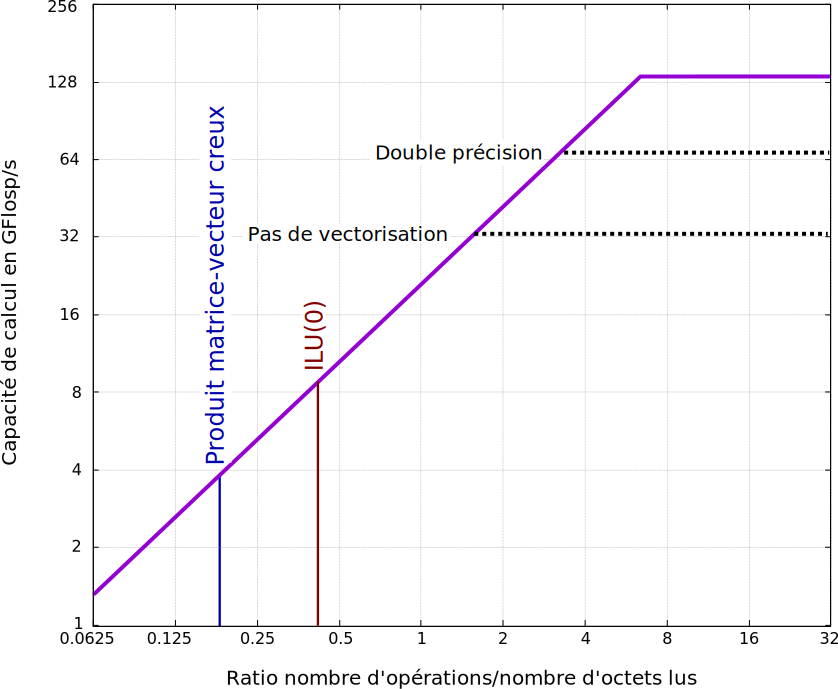
\includegraphics[width=0.8\textwidth]{roofline_rostand}
  \caption{Roofline model de Rostand avec les différents produit matrice vecteur creux.}
  \label{fig:roofline_rostand}
\end{figure}


% -------------------------------
\subsubsection{Mémoire distribuée}
Le produit matrice vecteur creux, que j'abrégerai SpMV pour le reste des résultats, est un algorithme qui se parallélise très bien en mémoire partagée.
%
Nous pouvons donc estimer que la performance atteinte en mémoire distribuée est une borne maximale à atteindre en mémoire partagée.
%
En effet, de par sa nature distribuée, les pénalités mémoires NUMA sont minimales.
%
Le roofline model prédit un algorithme limité en performance par la bande passante mémoire.
%
Or, cette bande passante mémoire est partagée entre les coeurs d'un même banc NUMA.
%
L'accélération obtenue sera donc limité par la bande passante mémoire.
%
Sur la machine rostand, la bande passante mémoire limite grandement cette accélération (fig.~\ref{fig:res_spmv_mpi_rostand}).
%
Avec un cas à 8 variables primaires, nous obtenons une accélération maximal de 3,8.
%
La capacité de calcul mesuré avec 12 coeurs est de 4,96~GFlops, cela correspond à la prédiction du roofline model.


%   (-_-)   %
\begin{figure}[t!]
  \centering
  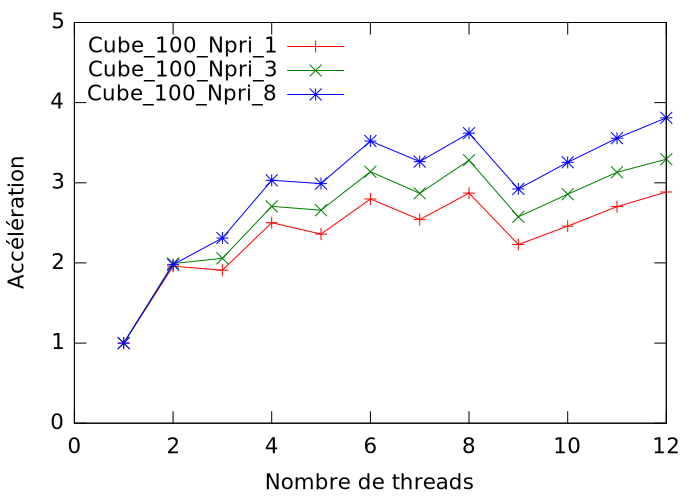
\includegraphics[width=0.7\textwidth]{res_spmv_mpi}
  \caption{Accélération du produit matrice vecteur creux sur Rostand en mémoire distribuée.}
  \label{fig:res_spmv_mpi_rostand}
\end{figure}



Sur Manumanu, nous avons beaucoup plus de banc NUMA, ce qui signifie que nous aurons plus de bande passante mémoire à notre disposition.
%
Nous pouvons donc espérer avoir de meilleurs résultats que sur Rostand.
%
Il faut aussi prendre en compte une bande passante mémoire plus élevée sur les banc NUMA de Manumanu que sur ceux de Rostand.
%
Les processus MPI sont alloués en mode compact, c'est à dire qu'ils sont distribués de façon à utiliser un minimum de noeuds NUMA.
%
Sur 1 banc NUMA, nous avons une accélération de 5 avec 8 variables primaires (fig~\ref{fig:res_spmv_mpi_manu}).
%
Cette accélération monte à 110 avec l'utilisation des 20 bancs NUMA et des 160 coeurs.


%   (-_-)   %
\begin{figure}[t!]
  \centering
  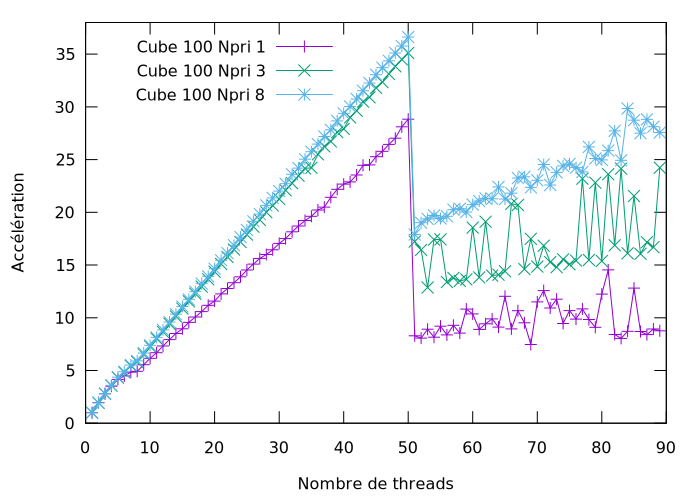
\includegraphics[width=0.7\textwidth]{res_spmv_mpi_manu}
  \caption{Accélération du produit matrice vecteur creux sur Manumanu en mémoire distribuée.}
  \label{fig:res_spmv_mpi_manumanu}
\end{figure}

% -------------------------------
\subsubsection{First touch}
Nous allons maintenant nous concentrer sur la parallélisation du SpMV en mémoire partagée.
%
La mémoire est allouée sur un seul banc NUMA et le travail est partagée par une directive {\em \#pragma omp parallel for}.
%
Sur la machine Rostand, nous obtenons difficilement une accélération de 2,5 sur 12 coeurs en ayant 8 variables primaires (Fig.~\ref{fig:res_spmv_ft_rostand}).
%
Cette accélération descend à 1,9 en ayant 1 variable primaire, toujours sur 12 coeurs de calcul.
%
Ces résultats sont à comparer avec ceux obtenues en mémoire distribuée.
%
Nous n'obtenons que 65~\% de la puissance maximale que nous devrions avoir.
%
Le SpMV étant limité par la bande passante mémoire, l'utilisation d'un seul banc NUMA pour les accès mémoire ne nous permet pas d'exploiter toute la puissance de la machine.




Sur la machine Manumanu, ces effets sont amplifiés (Fig.~\ref{fig:res_spmv_ft_manu}).
%
Nous obtenons les meilleures performances en utilisant 8 coeurs avec une accélération de 5-6.
%
Utiliser plus de 8 coeurs pour effectuer le SpMV fait perdre du temps, les données étant toute sur le premier banc NUMA, nous utilisons uniquement la bande passante de ce banc avec des latences d'accès plus ou moins longues.
%
Les résultats en mémoire distribuée sont meilleurs.
%
Pour obtenir les mêmes performances qu'en mémoire distribuée, nous devons optimiser les accès mémoire.

% -------------------------------
\subsubsection{Interleave}
Pour diminuer les effets NUMA, nous pouvons utiliser la politique d'allocation interleave.
%
Cette politique va distribuer uniformément les pages mémoires sur les différents bancs NUMA.
%
Nous allons donc augmenter la bande passante mémoire en ne modifiant que la latence mémoire moyenne.
%
Sur Rostand, nous obtenons un gain de performance d'environ 20~\% mais les performances sont toujours en dessous des performances obtenues en mémoire partagée (Fig.~\ref{fig:res_spmv_interleave_rostand}).

%   (-_-)   %
\begin{figure}[t!]
  \centering
  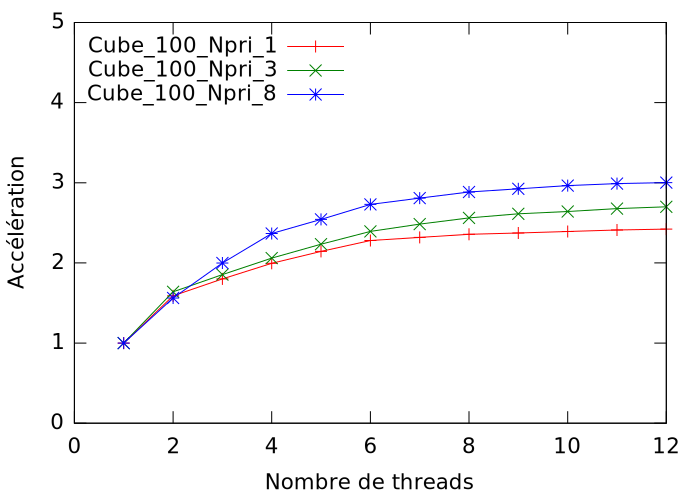
\includegraphics[width=0.7\textwidth]{res_spmv_interleave}
  \caption{Accélération du produit matrice vecteur creux sur Rostand en mémoire partagée avec une politique d'allocation interleave.}
  \label{fig:res_spmv_interleave_rostand}
\end{figure}

Sur Manumanu, on obtient de bons résultats jusqu'à 16 coeurs (Fig.~\ref{fig:res_spmv_interleave_manumanu}).
%
Au delà, nous commençons à utiliser le SGI$^\registered$ NUMAlink$^{\rm TM}$\cite{numalink} et les temps de latence des accès mémoire augmentent.
%
En effet, la majorité des accès mémoire se font sur des bancs NUMA distant.
%
Au final, les résultats de l'allocation interleave sur Manumanu sont proches des résultats de l'allocation first touch.
%
Ce n'est donc pas la bonne solution pour exploiter les performances de cette machine.

%   (-_-)   %
\begin{figure}[t!]
  \centering
  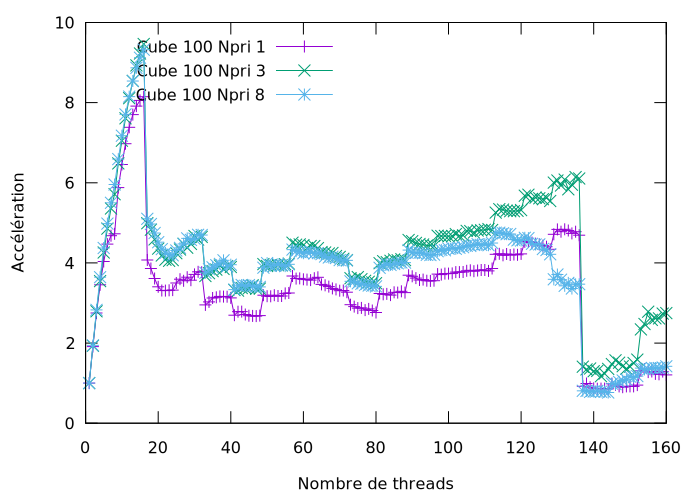
\includegraphics[width=0.7\textwidth]{res_spmv_interleave_manu}
  \caption{Accélération du produit matrice vecteur creux sur Manumanu en mémoire partagée avec une politique d'allocation interleave.}
  \label{fig:res_spmv_interleave_manumanu}
\end{figure}

%-------------------------------
\subsection{NATaS}
\`A la différence des autres ordonnanceurs, NATaS va tenir compte de l'affinité NUMA des tâches.
%
Cette affinité a été définit par Taggre de tel sorte à équilibrer la charge sur les différents banc NUMA.
%



Sur plusieurs bancs NUMA, NATaS offre des meilleurs performances que l'ordonnanceur OpenMP même avec l'allocation mémoire interleaved.
%
{\em Donner résultat manumanu}
%

%-------------------------------




%%%%%%%%%%%%%%%%
% SpMV
%%%%%%%%%%%%%%%%

%   (-_-)   %
\begin{figure}[!h]
     \begin{center}
        \subfigure[First touch.]{
          \label{fig:res_spmv_ft_rostand}
          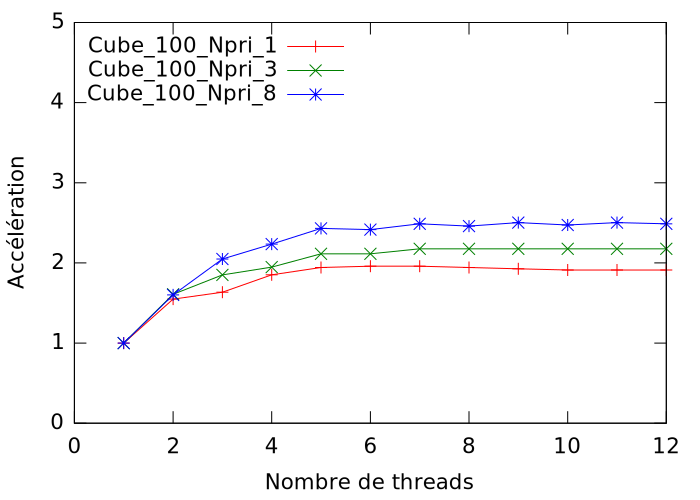
\includegraphics[width=0.48\textwidth]{res_spmv_omp}
        }
        \subfigure[Interleave.]{
          \label{fig:res_spmv_inter_rostand}
          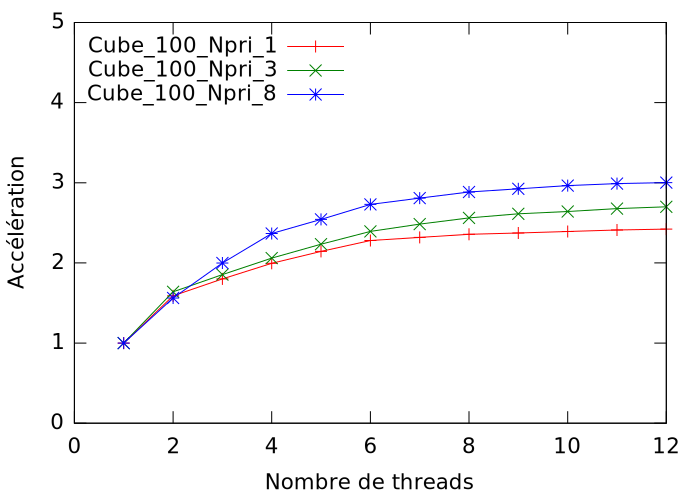
\includegraphics[width=0.48\textwidth]{res_spmv_interleave}
        }

        \subfigure[NATaS.]{
          \label{fig:res_spmv_nas_rostand}
          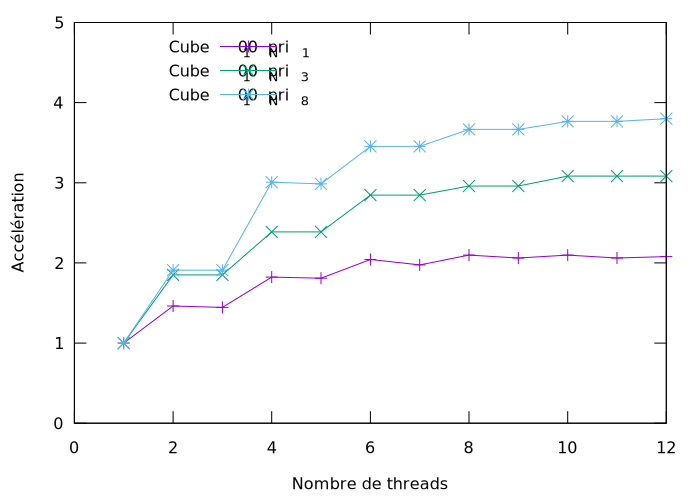
\includegraphics[width=0.48\textwidth]{res_spmv_nas}
        }
        \subfigure[MPI.]{
          \label{fig:res_spmv_mpi_rostand}
          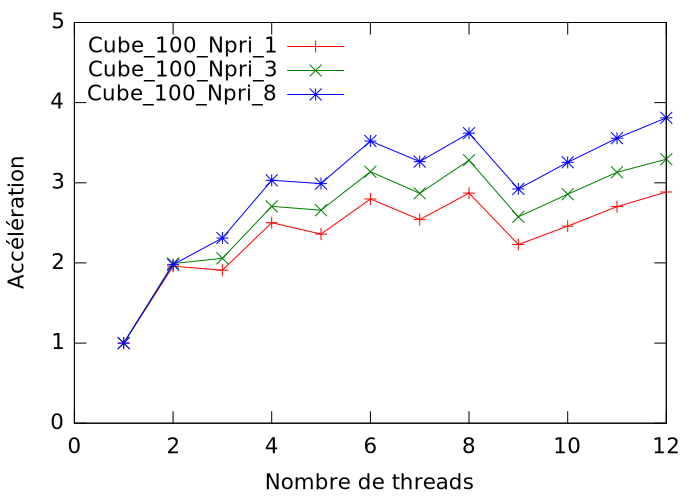
\includegraphics[width=0.48\textwidth]{res_spmv_mpi}
        }
    \end{center}
    \caption{Performances du produit matrice vecteur creux sur Rostand.}
\end{figure}



%   (-_-)   %
\begin{figure}[!h]
     \begin{center}
        \subfigure[First touch.]{
          \label{fig:res_spmv_ft_manu}
          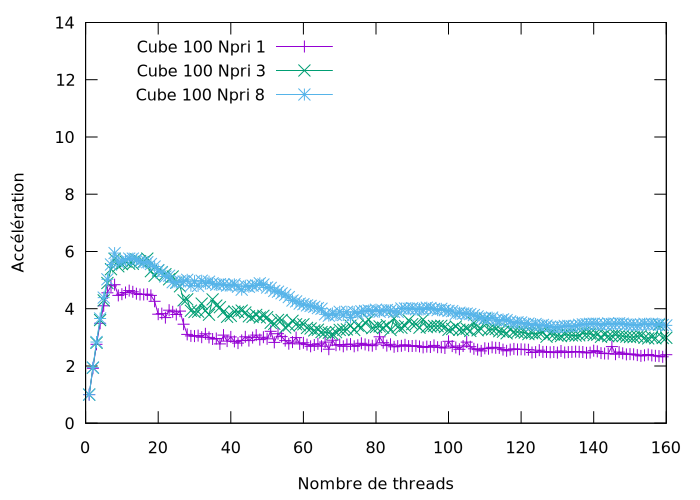
\includegraphics[width=0.48\textwidth]{res_spmv_omp_manu}
        }
        \subfigure[Interleave.]{
          \label{fig:res_spmv_inter_manu}
          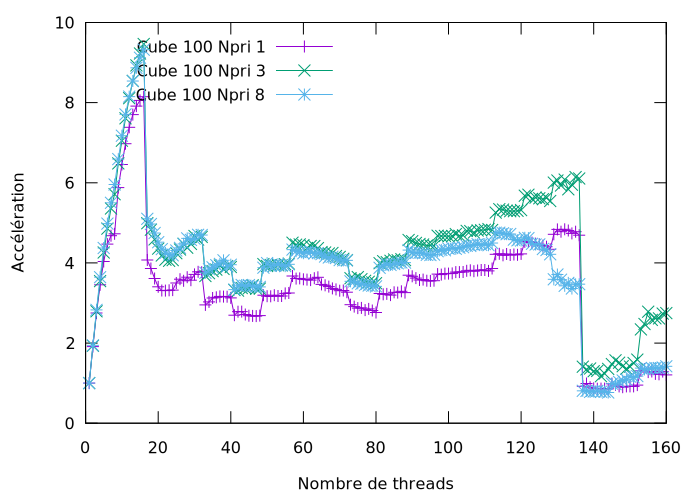
\includegraphics[width=0.48\textwidth]{res_spmv_interleave_manu}
        }

        \subfigure[NATaS.]{
          \label{fig:res_spmv_nas_manu}
          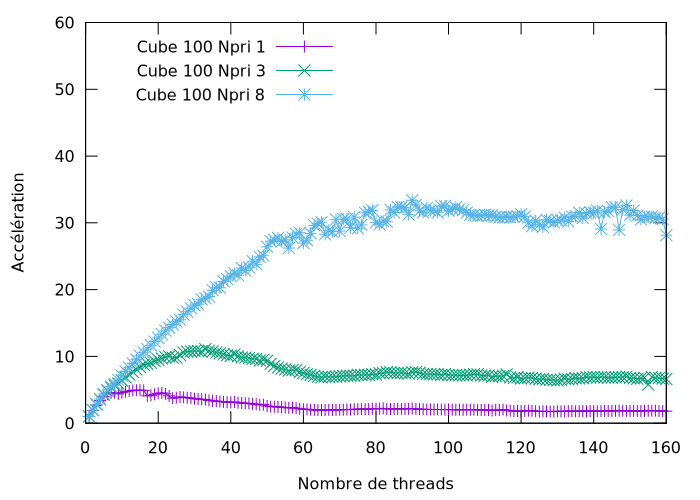
\includegraphics[width=0.48\textwidth]{res_spmv_nas_manu}
        }
        \subfigure[MPI.]{
          \label{fig:res_spmv_mpi_manu}
          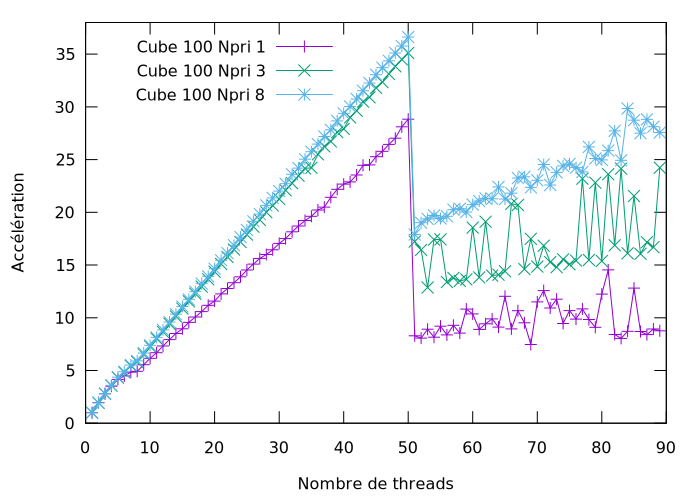
\includegraphics[width=0.48\textwidth]{res_spmv_mpi_manu}
        }
    \end{center}
    \caption{Performances du produit matrice vecteur creux sur Manumanu.}
\end{figure}





%-------------------------------
\subsubsection{\'Equilibrage automatique NUMA}
Les noyaux Linux récents proposent un équilibrage de charge automatique des pages mémoires.
%
Malheureusement, nous ne pouvons pas utiliser les grappes de serveurs à notre disposition pour tester cette fonctionnalité.
%
La version de Linux disponible sur ces machines n'est pas assez récente, la fonctionnalité AutoNUMA n'est apparue que dans la version 3.13 du noyau.
%
\`A la place, nous allons utiliser une machine de bureau contenant deux processeurs Intel Xeon X5660, chaque banc NUMA dispose de 6 coeurs de calculs et de 24~Go de mémoire vive.
%
La version de Linux utilisée est la 3.18.

Cette méthode ne fonctionne que lorsque le programme est exécuté suffisamment longtemps pour avoir le temps d'analyser toute la mémoire utilisée.
%
Nous allons chercher l'accélération maximale que nous pouvons atteindre avec cette solution.
%
Il ne nous est donc pas utile de faire varier le nombre de coeurs de calcul, nous utiliserons les 12 coeurs de calcul de la machine.
%
Nous allons plutôt faire varier le nombre de SpMV pour faire varier le temps d'exécution du programme et laisser au noyau assez de temps pour déplacer les pages.

%   (-_-)   %
\begin{figure}
  \centering
  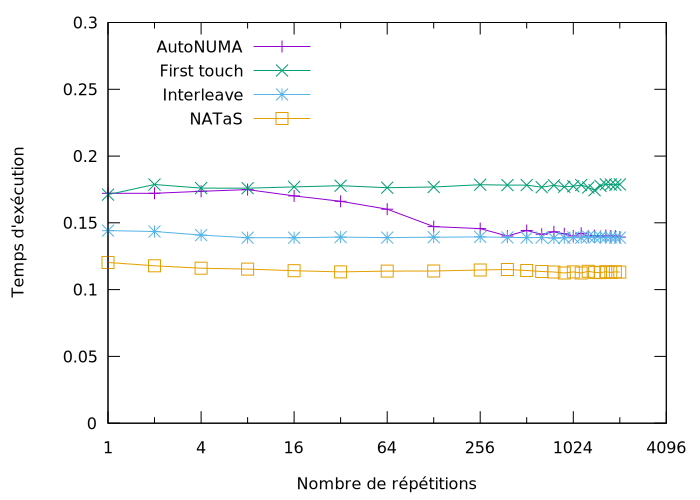
\includegraphics[width=0.7\textwidth]{res_spmv_frep}
  \caption{Temps d'un produit matrice vecteur creux sur Linux 3.18 en mémoire partagée avec 12 coeurs. Nous utilisons une matrice représentant un cube 100 avec 8 variables primaires.}
  \label{fig:res_spmv_frep}
\end{figure}

Avec un nombre de répétitions faibles, AutoNUMA donne les mêmes performances que l'allocation first touch (Fig.~\ref{fig:res_spmv_frep}).
%
Au bout de 8 répétitions, soit environ 1,36~seconde, nous commençons à voir une amélioration des performances.
%
Vers 384 répétitions, soit environ 1 minute, nous obtenons la performance crête d'AutoNUMA qui correspond aussi à la performance obtenue avec l'allocation interleave.
%
Il est nécessaire de rappeler que l'allocation interleave donnait de bonnes performances avec l'utilisation de 2 bancs NUMA.
%
Les meilleurs résultats sont obtenus avec NATaS.
%
Il serait aussi intéressant de tester la méthode AutoNUMA sur Manumanu en utilisant plus de 2 bancs NUMA, nous pourrions savoir si les résultats sont meilleurs qu'avec NATaS.
%
Malheureusement, nous nous ne pouvons pas changer le noyau utilisé sur cette machine.

% -------------------------------
